\section{Design}

The Stack consists of a series of modules tied together with a common
input control and output transmission multiplexer (figure
\ref{overview.simple}).
 
\begin{figure}
\begin{centering}
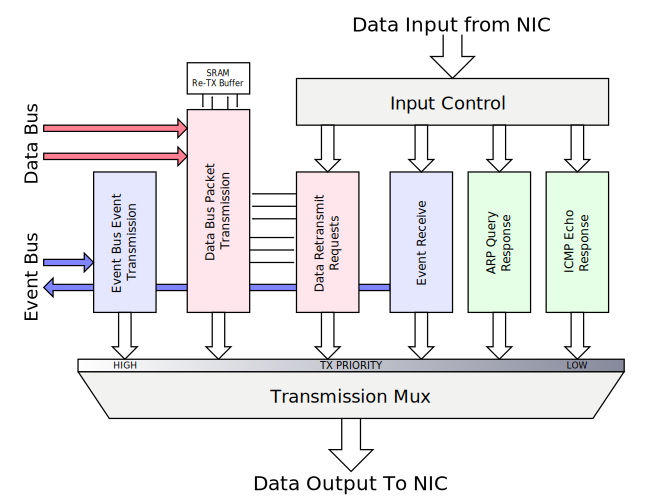
\includegraphics[scale=0.8]{overview.simple.svg}
\end{centering}
\caption{An overview of the Soma Network Stack architecture}
\label{overview.simple}
\end{figure}

There are six packet processing modules, the Input Control, and the
Transmission Multiplexer. Each packet processing module, pending an
arbitration step with the transmission multiplexer, directly passes
its buffer contents to the soma network stack.

The \textbf{Transmission Multiplexer} handles arbitration and
multiplexing the output of each packet processing module with the
Network Interface. Each packet processing module asserts a signal to
indicate pending data, and the transmission multiplexer grants access
to the network interface in a prioritized scheme which gives
mission-critical data (event and data bus transmission) priority at
the expense of debug (ARP and ICMP) packets.

The \textbf{Input Control} subsystem parses incoming frames from the
NIC and selectively engages the Data Retransmit Request, Event
Receive, ARP Query Response, or ICMP Echo Response packet processing
module. The associated module then has exclusive read access to the
received packet stored in the Input Control, and uses this packet to
build up its response. The packet processing module only releases
control back to the Input Control module when it has completed
transmission of its internal packet.

Soma Event Bus transmission is handled via the \textbf{Event Bus
  Transmission} packet processing module, which aggregates inbound
events according to the Soma Network Protocol. The resulting broadcast
frames can be up to 1100 bytes in length.

Event reception, handled by the \textbf{Event Receive} packet
processing module, is somewhat more complex due to the
request-response nature of inbound events in the network protocol.

The importance of error-free data transmission to the soma system
motivated the design of the \textbf{Data Bus Packet Transmission}
packet processing module. Here we use a 512 kB buffer to store
recently-transmitted packets, and add on a unique source/type-specific
sequence ID.

The \textbf{Data Request Transmission} module receives a request for a
retransmission and asks the Data Bus Packet Transmission module to
retrieve that packet. If the packet is still in the buffer, it is
transmitted out the interface.

The necessity of answering Address Resolution Protocol (ARP) queries motivated the simple \textbf{ARP Who-Has Query Response } Packet Processing Module. The need for diagnostic response tools lead to the creation of the \textbf{ICMP Echo Response} Packet Processing Module. 


